% One-slide talk (O-slide). Рисунок: python code/oslide/main.py --plot
\documentclass[aspectratio=169,10pt]{beamer}
\usepackage{iftex}
\ifPDFTeX
  \usepackage[T2A]{fontenc}
  \usepackage[utf8]{inputenc}
  \usepackage[russian]{babel}
\else
  \usepackage{fontspec}
  \setsansfont{DejaVu Sans}[Scale=0.92]
  \usepackage[russian,provide=*]{babel}
\fi
\usepackage{graphicx}
\usecolortheme{beaver}
\setbeamertemplate{navigation symbols}{}
\setbeamersize{text margin left=0.45cm,text margin right=0.45cm}
\definecolor{runA}{HTML}{2A78D6}
\definecolor{runB}{HTML}{EB6834}

\begin{document}
\begin{frame}{Точность теряется после детектора огибающей}
\vspace{-0.9em}
{\small Декодер Petrosyan et al.\ (2022): интерпретируемый ED-блок $\to$ BiLSTM $\to$ классификатор.}

\vspace{0.2em}
\begin{columns}[T,onlytextwidth]
\begin{column}{0.6\textwidth}
  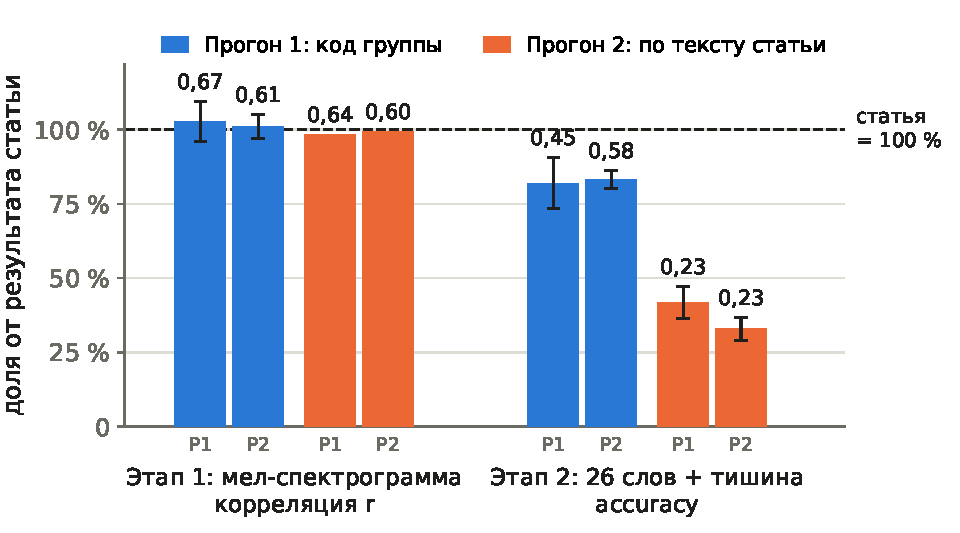
\includegraphics[width=\linewidth]{figs/oslide.pdf}
\end{column}
\begin{column}{0.38\textwidth}
\scriptsize
\textbf{Обозначения}\\[0.1em]
Этап 1: окно 1\,с iEEG $\to$ 40 лог-мел полос; $r$ Пирсона на test.\\
Этап 2: признаки этапа 1 $\to$ 27 классов; случайно 3,7\,\%.\\
P1~--- sEEG, P2~--- ЭКоГ. Планки: {\color{runA}$\pm$SD по 6 фолдам}, {\color{runB}$\pm$SE}.

\vspace{0.4em}
\textbf{Результат}\\[0.1em]
Этап 1 = статья в обоих прогонах (98--103\,\%).\\
Этап 2: 82--83\,\% и 33--42\,\% от статьи.

\vspace{0.4em}
\textbf{Чем различаются прогоны}\\[0.1em]
{\color{runA}1}: 6/8 каналов, фильтр с нулевой фазой (видит будущее), 6-fold CV.\\
{\color{runB}2}: 30/42 канала, причинный фильтр, как в статье; одно разбиение.\\
Контроль: причинный фильтр в прогоне~1 $\Rightarrow$ 47\,\%$\to$22\,\% (P1, 1 фолд).
\end{column}
\end{columns}

\vspace{-0.1em}
\begin{block}{Следствие}
\footnotesize При одинаковом $r$ точность слов различается вдвое: этап 1 не измеряет того, что нужно классификатору.
Замену BiLSTM на причинную TCN сравниваю по этапу 2 в причинном режиме; базовая линия~--- прогон 2.
\end{block}
\vspace{-0.5em}
{\tiny\color{gray} Акустическая утечка (microphone effect) ещё не проверена. Код: \texttt{code/oslide}, github.com/Stocck/subject-prior.}
\end{frame}
\end{document}
